\documentclass[twoside]{book}

% Packages required by doxygen
\usepackage{calc}
\usepackage{doxygen}
\usepackage{graphicx}
\usepackage[utf8]{inputenc}
\usepackage{makeidx}
\usepackage{multicol}
\usepackage{multirow}
\usepackage{fixltx2e}
\PassOptionsToPackage{warn}{textcomp}
\usepackage{textcomp}
\usepackage[nointegrals]{wasysym}
\usepackage[table]{xcolor}

% Font selection
\usepackage[T1]{fontenc}
\usepackage{mathptmx}
\usepackage[scaled=.90]{helvet}
\usepackage{courier}
\usepackage{amssymb}
\usepackage{sectsty}
\renewcommand{\familydefault}{\sfdefault}
\allsectionsfont{%
  \fontseries{bc}\selectfont%
  \color{darkgray}%
}
\renewcommand{\DoxyLabelFont}{%
  \fontseries{bc}\selectfont%
  \color{darkgray}%
}
\newcommand{\+}{\discretionary{\mbox{\scriptsize$\hookleftarrow$}}{}{}}

% Page & text layout
\usepackage{geometry}
\geometry{%
  a4paper,%
  top=2.5cm,%
  bottom=2.5cm,%
  left=2.5cm,%
  right=2.5cm%
}
\tolerance=750
\hfuzz=15pt
\hbadness=750
\setlength{\emergencystretch}{15pt}
\setlength{\parindent}{0cm}
\setlength{\parskip}{0.2cm}
\makeatletter
\renewcommand{\paragraph}{%
  \@startsection{paragraph}{4}{0ex}{-1.0ex}{1.0ex}{%
    \normalfont\normalsize\bfseries\SS@parafont%
  }%
}
\renewcommand{\subparagraph}{%
  \@startsection{subparagraph}{5}{0ex}{-1.0ex}{1.0ex}{%
    \normalfont\normalsize\bfseries\SS@subparafont%
  }%
}
\makeatother

% Headers & footers
\usepackage{fancyhdr}
\pagestyle{fancyplain}
\fancyhead[LE]{\fancyplain{}{\bfseries\thepage}}
\fancyhead[CE]{\fancyplain{}{}}
\fancyhead[RE]{\fancyplain{}{\bfseries\leftmark}}
\fancyhead[LO]{\fancyplain{}{\bfseries\rightmark}}
\fancyhead[CO]{\fancyplain{}{}}
\fancyhead[RO]{\fancyplain{}{\bfseries\thepage}}
\fancyfoot[LE]{\fancyplain{}{}}
\fancyfoot[CE]{\fancyplain{}{}}
\fancyfoot[RE]{\fancyplain{}{\bfseries\scriptsize Generated on Sun Dec 7 2014 14\+:31\+:19 for S\+E\+M\+T-\/\+O\+Care by Doxygen }}
\fancyfoot[LO]{\fancyplain{}{\bfseries\scriptsize Generated on Sun Dec 7 2014 14\+:31\+:19 for S\+E\+M\+T-\/\+O\+Care by Doxygen }}
\fancyfoot[CO]{\fancyplain{}{}}
\fancyfoot[RO]{\fancyplain{}{}}
\renewcommand{\footrulewidth}{0.4pt}
\renewcommand{\chaptermark}[1]{%
  \markboth{#1}{}%
}
\renewcommand{\sectionmark}[1]{%
  \markright{\thesection\ #1}%
}

% Indices & bibliography
\usepackage{natbib}
\usepackage[titles]{tocloft}
\setcounter{tocdepth}{3}
\setcounter{secnumdepth}{5}
\makeindex

% Hyperlinks (required, but should be loaded last)
\usepackage{ifpdf}
\ifpdf
  \usepackage[pdftex,pagebackref=true]{hyperref}
\else
  \usepackage[ps2pdf,pagebackref=true]{hyperref}
\fi
\hypersetup{%
  colorlinks=true,%
  linkcolor=blue,%
  citecolor=blue,%
  unicode%
}

% Custom commands
\newcommand{\clearemptydoublepage}{%
  \newpage{\pagestyle{empty}\cleardoublepage}%
}


%===== C O N T E N T S =====

\begin{document}

% Titlepage & ToC
\hypersetup{pageanchor=false,
             bookmarks=true,
             bookmarksnumbered=true,
             pdfencoding=unicode
            }
\pagenumbering{roman}
\begin{titlepage}
\vspace*{7cm}
\begin{center}%
{\Large S\+E\+M\+T-\/\+O\+Care }\\
\vspace*{1cm}
{\large Generated by Doxygen 1.8.7}\\
\vspace*{0.5cm}
{\small Sun Dec 7 2014 14:31:19}\\
\end{center}
\end{titlepage}
\clearemptydoublepage
\tableofcontents
\clearemptydoublepage
\pagenumbering{arabic}
\hypersetup{pageanchor=true}

%--- Begin generated contents ---
\chapter{S\+E\+M\+T-\/\+O\+Care}
\label{index}\hypertarget{index}{}\begin{DoxyAuthor}{Authors}
codejava.\+net 

 Modifiers\+: Bryan Connelly, Johnlee Alvarez 

 
\end{DoxyAuthor}
\begin{DoxyDate}{Date}
12/9/2014 

 ~\newline

\end{DoxyDate}
\hypertarget{index_intro}{}\section{Java Servlets}\label{index_intro}

\begin{DoxyItemize}
\item These Servlets are what allow Patients/\+Doctors to upload and download the records.
\item We determine whether or not you are a doctor or patient based on your login info ~\newline


 
\end{DoxyItemize}
\chapter{Hierarchical Index}
\section{Class Hierarchy}
This inheritance list is sorted roughly, but not completely, alphabetically\+:\begin{DoxyCompactList}
\item Http\+Servlet\begin{DoxyCompactList}
\item \contentsline{section}{net.\+codejava.\+upload.\+Servlet1}{\pageref{classnet_1_1codejava_1_1upload_1_1_servlet1}}{}
\item \contentsline{section}{net.\+codejava.\+upload.\+Servlet2}{\pageref{classnet_1_1codejava_1_1upload_1_1_servlet2}}{}
\item \contentsline{section}{net.\+codejava.\+upload.\+Servlet3}{\pageref{classnet_1_1codejava_1_1upload_1_1_servlet3}}{}
\end{DoxyCompactList}
\end{DoxyCompactList}

\chapter{Class Index}
\section{Class List}
Here are the classes, structs, unions and interfaces with brief descriptions\+:\begin{DoxyCompactList}
\item\contentsline{section}{\hyperlink{classnet_1_1codejava_1_1upload_1_1_servlet1}{net.\+codejava.\+upload.\+Servlet1} }{\pageref{classnet_1_1codejava_1_1upload_1_1_servlet1}}{}
\item\contentsline{section}{\hyperlink{classnet_1_1codejava_1_1upload_1_1_servlet2}{net.\+codejava.\+upload.\+Servlet2} }{\pageref{classnet_1_1codejava_1_1upload_1_1_servlet2}}{}
\item\contentsline{section}{\hyperlink{classnet_1_1codejava_1_1upload_1_1_servlet3}{net.\+codejava.\+upload.\+Servlet3} }{\pageref{classnet_1_1codejava_1_1upload_1_1_servlet3}}{}
\end{DoxyCompactList}

\chapter{Class Documentation}
\hypertarget{classnet_1_1codejava_1_1upload_1_1_servlet1}{\section{net.\+codejava.\+upload.\+Servlet1 Class Reference}
\label{classnet_1_1codejava_1_1upload_1_1_servlet1}\index{net.\+codejava.\+upload.\+Servlet1@{net.\+codejava.\+upload.\+Servlet1}}
}
Inheritance diagram for net.\+codejava.\+upload.\+Servlet1\+:\begin{figure}[H]
\begin{center}
\leavevmode
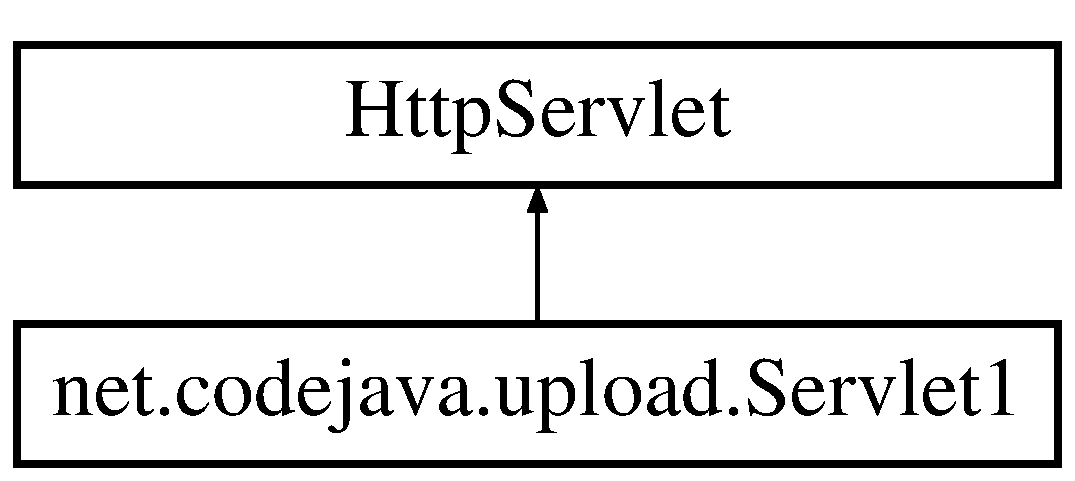
\includegraphics[height=2.000000cm]{classnet_1_1codejava_1_1upload_1_1_servlet1}
\end{center}
\end{figure}
\subsection*{Protected Member Functions}
\begin{DoxyCompactItemize}
\item 
void \hyperlink{classnet_1_1codejava_1_1upload_1_1_servlet1_ac163d46545f634472456bd749b91a7c9}{do\+Post} (Http\+Servlet\+Request request, Http\+Servlet\+Response response)  throws Servlet\+Exception, I\+O\+Exception 
\item 
void \hyperlink{classnet_1_1codejava_1_1upload_1_1_servlet1_ab38ac3551f31e1b69eabfae8cdb885f8}{do\+Get} (Http\+Servlet\+Request request, Http\+Servlet\+Response response)  throws Servlet\+Exception, I\+O\+Exception 
\end{DoxyCompactItemize}


\subsection{Detailed Description}
A Java servlet that handles file upload and download from client. \begin{DoxyAuthor}{Author}
www.\+codejava.\+net 

 Modifiers\+: Bryan Connelly, Johnlee Alvarez 

 
\end{DoxyAuthor}


\subsection{Member Function Documentation}
\hypertarget{classnet_1_1codejava_1_1upload_1_1_servlet1_ab38ac3551f31e1b69eabfae8cdb885f8}{\index{net\+::codejava\+::upload\+::\+Servlet1@{net\+::codejava\+::upload\+::\+Servlet1}!do\+Get@{do\+Get}}
\index{do\+Get@{do\+Get}!net\+::codejava\+::upload\+::\+Servlet1@{net\+::codejava\+::upload\+::\+Servlet1}}
\subsubsection[{do\+Get}]{\setlength{\rightskip}{0pt plus 5cm}void net.\+codejava.\+upload.\+Servlet1.\+do\+Get (
\begin{DoxyParamCaption}
\item[{Http\+Servlet\+Request}]{request, }
\item[{Http\+Servlet\+Response}]{response}
\end{DoxyParamCaption}
) throws Servlet\+Exception, I\+O\+Exception\hspace{0.3cm}{\ttfamily [inline]}, {\ttfamily [protected]}}}\label{classnet_1_1codejava_1_1upload_1_1_servlet1_ab38ac3551f31e1b69eabfae8cdb885f8}

\begin{DoxyItemize}
\item This method handles file upload via H\+T\+T\+P G\+E\+T method
\item Download path is set from an absolute path on Local Disk
\item With more time we would have implemented a drop-\/down menu to select which file you wanted to download \begin{DoxyReturn}{Returns}
The file that is stored in the Download path 
\end{DoxyReturn}

\end{DoxyItemize}\hypertarget{classnet_1_1codejava_1_1upload_1_1_servlet1_ac163d46545f634472456bd749b91a7c9}{\index{net\+::codejava\+::upload\+::\+Servlet1@{net\+::codejava\+::upload\+::\+Servlet1}!do\+Post@{do\+Post}}
\index{do\+Post@{do\+Post}!net\+::codejava\+::upload\+::\+Servlet1@{net\+::codejava\+::upload\+::\+Servlet1}}
\subsubsection[{do\+Post}]{\setlength{\rightskip}{0pt plus 5cm}void net.\+codejava.\+upload.\+Servlet1.\+do\+Post (
\begin{DoxyParamCaption}
\item[{Http\+Servlet\+Request}]{request, }
\item[{Http\+Servlet\+Response}]{response}
\end{DoxyParamCaption}
) throws Servlet\+Exception, I\+O\+Exception\hspace{0.3cm}{\ttfamily [inline]}, {\ttfamily [protected]}}}\label{classnet_1_1codejava_1_1upload_1_1_servlet1_ac163d46545f634472456bd749b91a7c9}

\begin{DoxyItemize}
\item This method handles file upload via H\+T\+T\+P P\+O\+S\+T method
\item The upload path is determined as a location on local disk
\item Allows you to select which file you want to upload with drop-\/down menu \begin{DoxyReturn}{Returns}
Message stating if the upload was successful 
\end{DoxyReturn}

\end{DoxyItemize}

The documentation for this class was generated from the following file\+:\begin{DoxyCompactItemize}
\item 
Upload\+Servlet\+App/src/net/codejava/upload/Servlet1.\+java\end{DoxyCompactItemize}

\hypertarget{classnet_1_1codejava_1_1upload_1_1_servlet2}{\section{net.\+codejava.\+upload.\+Servlet2 Class Reference}
\label{classnet_1_1codejava_1_1upload_1_1_servlet2}\index{net.\+codejava.\+upload.\+Servlet2@{net.\+codejava.\+upload.\+Servlet2}}
}
Inheritance diagram for net.\+codejava.\+upload.\+Servlet2\+:\begin{figure}[H]
\begin{center}
\leavevmode
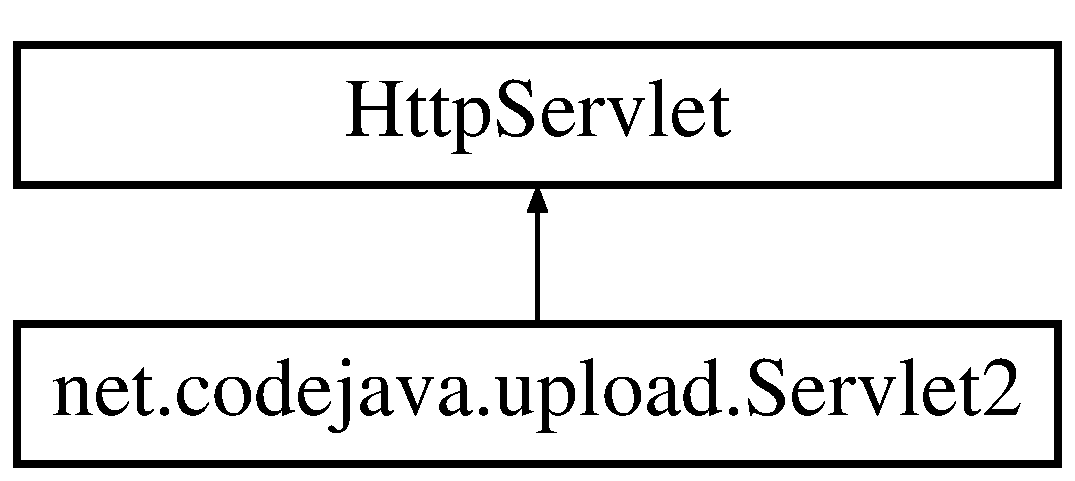
\includegraphics[height=2.000000cm]{classnet_1_1codejava_1_1upload_1_1_servlet2}
\end{center}
\end{figure}
\subsection*{Protected Member Functions}
\begin{DoxyCompactItemize}
\item 
void \hyperlink{classnet_1_1codejava_1_1upload_1_1_servlet2_a0af557e85b8bd04e4be725302794ea77}{do\+Post} (Http\+Servlet\+Request request, Http\+Servlet\+Response response)  throws Servlet\+Exception, I\+O\+Exception 
\item 
void \hyperlink{classnet_1_1codejava_1_1upload_1_1_servlet2_aba2b87d7d7e1a8824ee7f9b6544dd5f7}{do\+Get} (Http\+Servlet\+Request request, Http\+Servlet\+Response response)  throws Servlet\+Exception, I\+O\+Exception 
\end{DoxyCompactItemize}


\subsection{Detailed Description}
A Java servlet that handles file upload and download from client. \begin{DoxyAuthor}{Author}
www.\+codejava.\+net 

 Modifiers\+: Bryan Connelly, Johnlee Alvarez 

 
\end{DoxyAuthor}


\subsection{Member Function Documentation}
\hypertarget{classnet_1_1codejava_1_1upload_1_1_servlet2_aba2b87d7d7e1a8824ee7f9b6544dd5f7}{\index{net\+::codejava\+::upload\+::\+Servlet2@{net\+::codejava\+::upload\+::\+Servlet2}!do\+Get@{do\+Get}}
\index{do\+Get@{do\+Get}!net\+::codejava\+::upload\+::\+Servlet2@{net\+::codejava\+::upload\+::\+Servlet2}}
\subsubsection[{do\+Get}]{\setlength{\rightskip}{0pt plus 5cm}void net.\+codejava.\+upload.\+Servlet2.\+do\+Get (
\begin{DoxyParamCaption}
\item[{Http\+Servlet\+Request}]{request, }
\item[{Http\+Servlet\+Response}]{response}
\end{DoxyParamCaption}
) throws Servlet\+Exception, I\+O\+Exception\hspace{0.3cm}{\ttfamily [inline]}, {\ttfamily [protected]}}}\label{classnet_1_1codejava_1_1upload_1_1_servlet2_aba2b87d7d7e1a8824ee7f9b6544dd5f7}

\begin{DoxyItemize}
\item This method handles file upload via H\+T\+T\+P G\+E\+T method
\item Download path is set from an absolute path on Local Disk
\item With more time we would have implemented a drop-\/down menu to select which file you wanted to download \begin{DoxyReturn}{Returns}
The file that is stored in the Download path 
\end{DoxyReturn}

\end{DoxyItemize}\hypertarget{classnet_1_1codejava_1_1upload_1_1_servlet2_a0af557e85b8bd04e4be725302794ea77}{\index{net\+::codejava\+::upload\+::\+Servlet2@{net\+::codejava\+::upload\+::\+Servlet2}!do\+Post@{do\+Post}}
\index{do\+Post@{do\+Post}!net\+::codejava\+::upload\+::\+Servlet2@{net\+::codejava\+::upload\+::\+Servlet2}}
\subsubsection[{do\+Post}]{\setlength{\rightskip}{0pt plus 5cm}void net.\+codejava.\+upload.\+Servlet2.\+do\+Post (
\begin{DoxyParamCaption}
\item[{Http\+Servlet\+Request}]{request, }
\item[{Http\+Servlet\+Response}]{response}
\end{DoxyParamCaption}
) throws Servlet\+Exception, I\+O\+Exception\hspace{0.3cm}{\ttfamily [inline]}, {\ttfamily [protected]}}}\label{classnet_1_1codejava_1_1upload_1_1_servlet2_a0af557e85b8bd04e4be725302794ea77}

\begin{DoxyItemize}
\item This method handles file upload via H\+T\+T\+P P\+O\+S\+T method
\item The upload path is determined as a location on local disk
\item Allows you to select which file you want to upload with drop-\/down menu \begin{DoxyReturn}{Returns}
Message stating if the upload was successful 
\end{DoxyReturn}

\end{DoxyItemize}

The documentation for this class was generated from the following file\+:\begin{DoxyCompactItemize}
\item 
Upload\+Servlet\+App/src/net/codejava/upload/Servlet2.\+java\end{DoxyCompactItemize}

\hypertarget{classnet_1_1codejava_1_1upload_1_1_servlet3}{\section{net.\+codejava.\+upload.\+Servlet3 Class Reference}
\label{classnet_1_1codejava_1_1upload_1_1_servlet3}\index{net.\+codejava.\+upload.\+Servlet3@{net.\+codejava.\+upload.\+Servlet3}}
}
Inheritance diagram for net.\+codejava.\+upload.\+Servlet3\+:\begin{figure}[H]
\begin{center}
\leavevmode
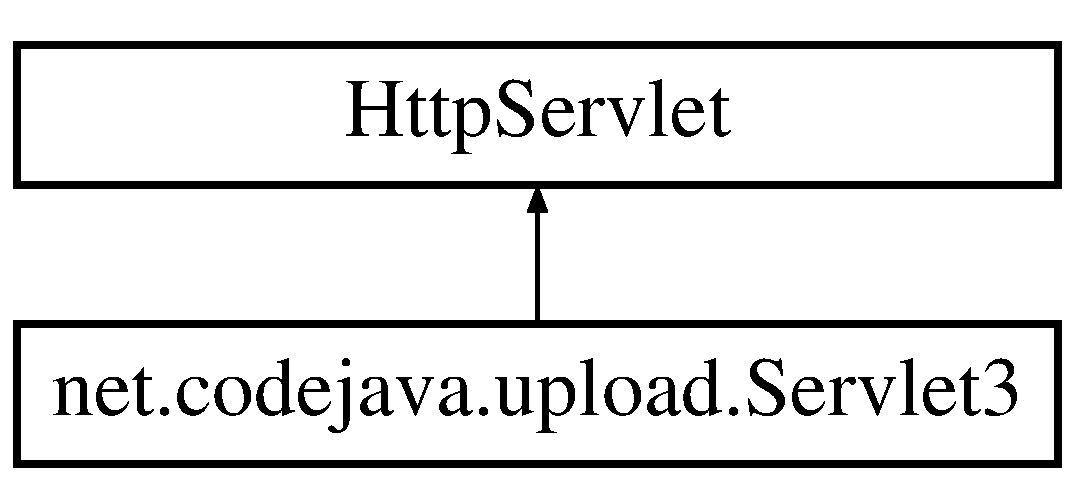
\includegraphics[height=2.000000cm]{classnet_1_1codejava_1_1upload_1_1_servlet3}
\end{center}
\end{figure}
\subsection*{Protected Member Functions}
\begin{DoxyCompactItemize}
\item 
void \hyperlink{classnet_1_1codejava_1_1upload_1_1_servlet3_a3148241befd6dd44828ded219d296ccb}{do\+Post} (Http\+Servlet\+Request request, Http\+Servlet\+Response response)  throws Servlet\+Exception, I\+O\+Exception 
\item 
void \hyperlink{classnet_1_1codejava_1_1upload_1_1_servlet3_a98ca5751af75437924fa30f9ac802702}{do\+Get} (Http\+Servlet\+Request request, Http\+Servlet\+Response response)  throws Servlet\+Exception, I\+O\+Exception 
\end{DoxyCompactItemize}


\subsection{Detailed Description}
A Java servlet that handles file upload and download from client. \begin{DoxyAuthor}{Author}
www.\+codejava.\+net 

 Modifiers\+: Bryan Connelly, Johnlee Alvarez 

 
\end{DoxyAuthor}


\subsection{Member Function Documentation}
\hypertarget{classnet_1_1codejava_1_1upload_1_1_servlet3_a98ca5751af75437924fa30f9ac802702}{\index{net\+::codejava\+::upload\+::\+Servlet3@{net\+::codejava\+::upload\+::\+Servlet3}!do\+Get@{do\+Get}}
\index{do\+Get@{do\+Get}!net\+::codejava\+::upload\+::\+Servlet3@{net\+::codejava\+::upload\+::\+Servlet3}}
\subsubsection[{do\+Get}]{\setlength{\rightskip}{0pt plus 5cm}void net.\+codejava.\+upload.\+Servlet3.\+do\+Get (
\begin{DoxyParamCaption}
\item[{Http\+Servlet\+Request}]{request, }
\item[{Http\+Servlet\+Response}]{response}
\end{DoxyParamCaption}
) throws Servlet\+Exception, I\+O\+Exception\hspace{0.3cm}{\ttfamily [inline]}, {\ttfamily [protected]}}}\label{classnet_1_1codejava_1_1upload_1_1_servlet3_a98ca5751af75437924fa30f9ac802702}

\begin{DoxyItemize}
\item This method handles file upload via H\+T\+T\+P G\+E\+T method
\item Download path is set from an absolute path on Local Disk
\item With more time we would have implemented a drop-\/down menu to select which file you wanted to download \begin{DoxyReturn}{Returns}
The file that is stored in the Download path 
\end{DoxyReturn}

\end{DoxyItemize}\hypertarget{classnet_1_1codejava_1_1upload_1_1_servlet3_a3148241befd6dd44828ded219d296ccb}{\index{net\+::codejava\+::upload\+::\+Servlet3@{net\+::codejava\+::upload\+::\+Servlet3}!do\+Post@{do\+Post}}
\index{do\+Post@{do\+Post}!net\+::codejava\+::upload\+::\+Servlet3@{net\+::codejava\+::upload\+::\+Servlet3}}
\subsubsection[{do\+Post}]{\setlength{\rightskip}{0pt plus 5cm}void net.\+codejava.\+upload.\+Servlet3.\+do\+Post (
\begin{DoxyParamCaption}
\item[{Http\+Servlet\+Request}]{request, }
\item[{Http\+Servlet\+Response}]{response}
\end{DoxyParamCaption}
) throws Servlet\+Exception, I\+O\+Exception\hspace{0.3cm}{\ttfamily [inline]}, {\ttfamily [protected]}}}\label{classnet_1_1codejava_1_1upload_1_1_servlet3_a3148241befd6dd44828ded219d296ccb}

\begin{DoxyItemize}
\item This method handles file upload via H\+T\+T\+P P\+O\+S\+T method
\item The upload path is determined as a location on local disk
\item Allows you to select which file you want to upload with drop-\/down menu \begin{DoxyReturn}{Returns}
Message stating if the upload was successful 
\end{DoxyReturn}

\end{DoxyItemize}

The documentation for this class was generated from the following file\+:\begin{DoxyCompactItemize}
\item 
Upload\+Servlet\+App/src/net/codejava/upload/Servlet3.\+java\end{DoxyCompactItemize}

%--- End generated contents ---

% Index
\newpage
\phantomsection
\addcontentsline{toc}{chapter}{Index}
\printindex

\end{document}
